\documentclass[a4paper]{article}

%% Language and font encodings
\usepackage[english]{babel}
\usepackage[utf8x]{inputenc}
\usepackage[T1]{fontenc}
\usepackage{makecell}

%% Sets page size and margins
\usepackage[a4paper,top=3cm,bottom=2cm,left=3cm,right=3cm,marginparwidth=1.75cm]{geometry}

%% Useful packages
\usepackage{amsmath}
\usepackage{amssymb}
\usepackage{amsfonts}
\usepackage[shortlabels]{enumitem}


\usepackage{graphicx}
\usepackage{tikz}
\usetikzlibrary{arrows.meta}

\usepackage[colorinlistoftodos]{todonotes}
\usepackage[colorlinks=true, allcolors=blue]{hyperref}

\usepackage{color}
\usepackage{url}

\title{Exam 1 - Practice Problems}
\author{CS 182 - Artificial Intelligence}

\begin{document}
\maketitle

\section{Search}

\begin{center}
\begin{tabular}{cc}
\parbox[c]{10cm}{\includegraphics[width =0.75\linewidth]{figs/search_graph.pdf} }
&
\begin{tabular}[h]{|c|c|c|c|}
\hline
Node &$h_1$ 	&	$h_2$ & $h_3$ \\
\hline
A 	& 	9.5 	&	10 & 14\\
B 	&	9	&	12	   & 13  \\
C 	&	8	&	10	   & 10   \\
D 	&	7	&	8	   & 8   \\
E 	&	1.5	&	1	   & 2 \\
F 	&	4	&	4.5	   & 4   \\
G 	&	0	&	0	   & 0   \\
\hline 
\end{tabular}
\end{tabular}
\end{center}

Consider the state space graph shown above.  A is the start state and
G is the goal state. The costs for each edge are shown on the graph.  Each edge can
be traversed in both directions. The table on the right shows three heuristics $h_1$, $h_2$ and $h_3$. 

\begin{enumerate}[(a)]
\item Are $h_1$, $h_2$ and $h_3$ consistent? Are they admissible? 

\vspace{4em}
% \textcolor{blue}{$h_1$ is both admissible and consistent. $h_2$ is not consistent (e.g. it increases by 2 from A to B). $h_3$ is consistent, but not admissible ($h_3(A)$ is 14 when the total minimal path cost is 13).}


\item For each of the following graph search strategies, mark which, if any, of the
listed paths it could return.   Note that for some search strategies
the specific path returned might depend on tie-breaking behavior.   In any such cases, make sure to mark
\emph{all} paths that could be returned under some tie-breaking scheme.

\vspace{.1in}
\begin{table}[!h]
\centering
\begin{tabular}{|l|c|c|c|}
\hline
Search Algorithm &  \textbf{A-B-D-G} & \textbf{A-C-D-G} &
\textbf{A-B-C-D-F-G} \\
\hline
Depth first search & & & \\
\hline
Breadth first search & & & \\
\hline
Uniform cost search & & & \\
\hline
A* search with heuristic $h_1$ & & &  \\
\hline
A* search with heuristic $h_2$ & & &  \\
\hline
A* search with heuristic $h_3$ & & & \\
\hline
\end{tabular}
\end{table}

\item Suppose you are completing the new heuristic function $h_4$ shown below.
All the values are fixed except $h_4(B)$. 

\begin{center}
\begin{tabular}{|c|c|c|c|c|c|c|c|}
\hline
Node & A & B & C & D & E & F & G \\
\hline
$h_4$& 10 & ?  & 9 & 7 & 1.5 & 4.5& 0 \\
\hline
\end{tabular}
\end{center}

For each of the following conditions, write the set of values that are possible for $h_4(B)$. (1) What values of $h_4(B)$ make $h_4$ admissible? (2) What values of $h_4(B)$ make $h_4$ consistent?

\newpage
% \textcolor{blue}{ (1) To make $h_4$ admissible, $h_4(B)$ has to be less than or equal to the actual optimal cost from B to goal G, which is the cost of path B-C-D-F-G, i.e. 12.  The answer is $0 \leq h_3(B) \leq 12$}

% \textcolor{blue}{
% (2) All the other nodes except node B satisfy the consistency conditions. The consistency conditions that do
% involve the state $B$ are:
% \begin{align*}
% h(A) \leq c(A, B) + h(B) \ \ \ & \ \ \ h(B) \leq c(B, A) + h(A)\\
% h(C) \leq c(C, B) + h(B) \ \ \ & \ \ \ h(B) \leq c(B, C) + h(C)\\
% h(D) \leq c(D, B) + h(B) \ \ \ & \ \ \ h(B) \leq c(B, D) + h(D)
% \end{align*}
% Filling in the numbers shows this results in the condition:
% $9 \leq h_3(B) \leq 10$}
\vspace{4em}
\item What values of $h_3(B)$ will cause A* graph search to expand node A, then node C, then node B, then node D in order?

\vspace{10em}
% \textcolor{blue}{
% In order to make A* graph search expand node A, then node C, then node B, suppose $h_3(B) = x$, we need
% \begin{align*}
% &1+x>13 \\
% &5+x<14 ~~~(expand~ B') ~~~ or ~~~ 1+x<14 ~~~ (expand~ B) 
% \end{align*}
% so we can get $12<h_3(B)<13$}

\end{enumerate}

% ------------------------------ADVERSARIAL
\section{Adversarial Search}

\begin{enumerate}[(a)]
\item Below you can see a search tree. Fill out the values of the nodes according to minimax search. What action would the agent take at the root?

\begin{center}
\begin{figure}[h!]
\centering
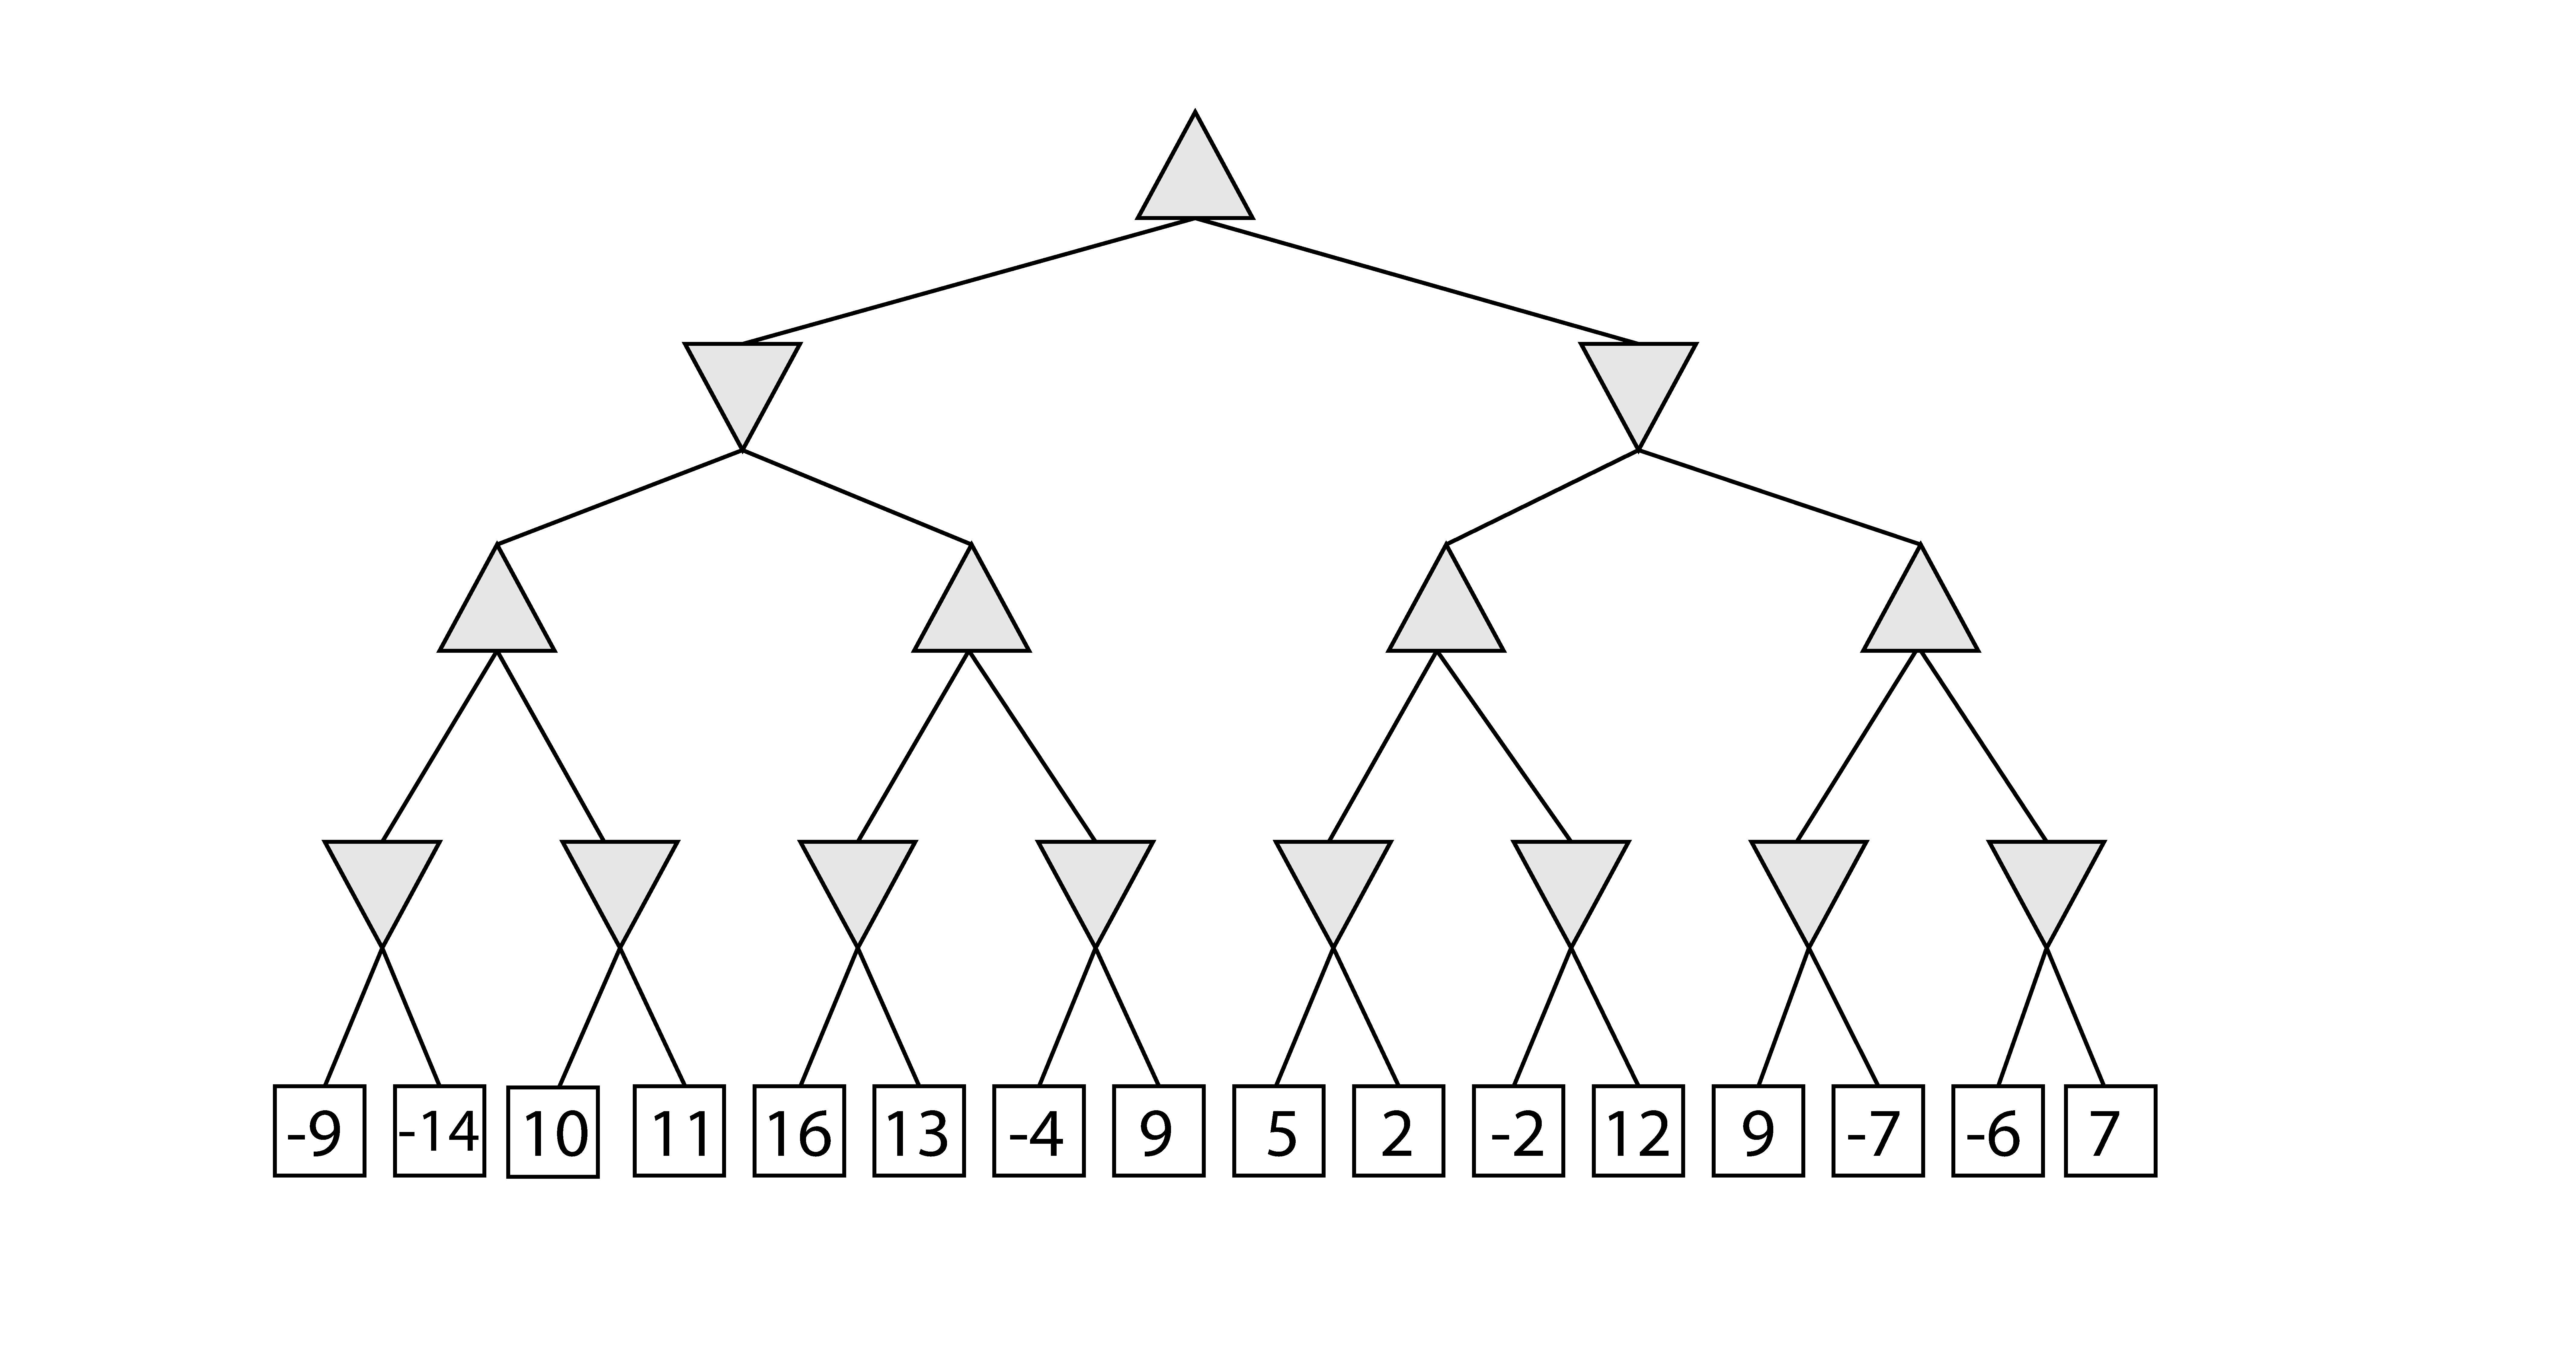
\includegraphics[width=1.25\textwidth]{figs/minmax}
\end{figure}
\end{center}

\newpage

% \textcolor{blue}{\textbf{Solution:}}

% \begin{center}
% \begin{figure}[h!]
% \centering
% \includegraphics[width=1\textwidth]{figs/alphabeta-sol}
% \end{figure}
% \end{center}

\item Mark the edges that would be pruned when using Alpha-Beta pruning? Also write the alpha and beta value as well as the value on each node. 

\begin{center}
\begin{figure}[h!]
\centering
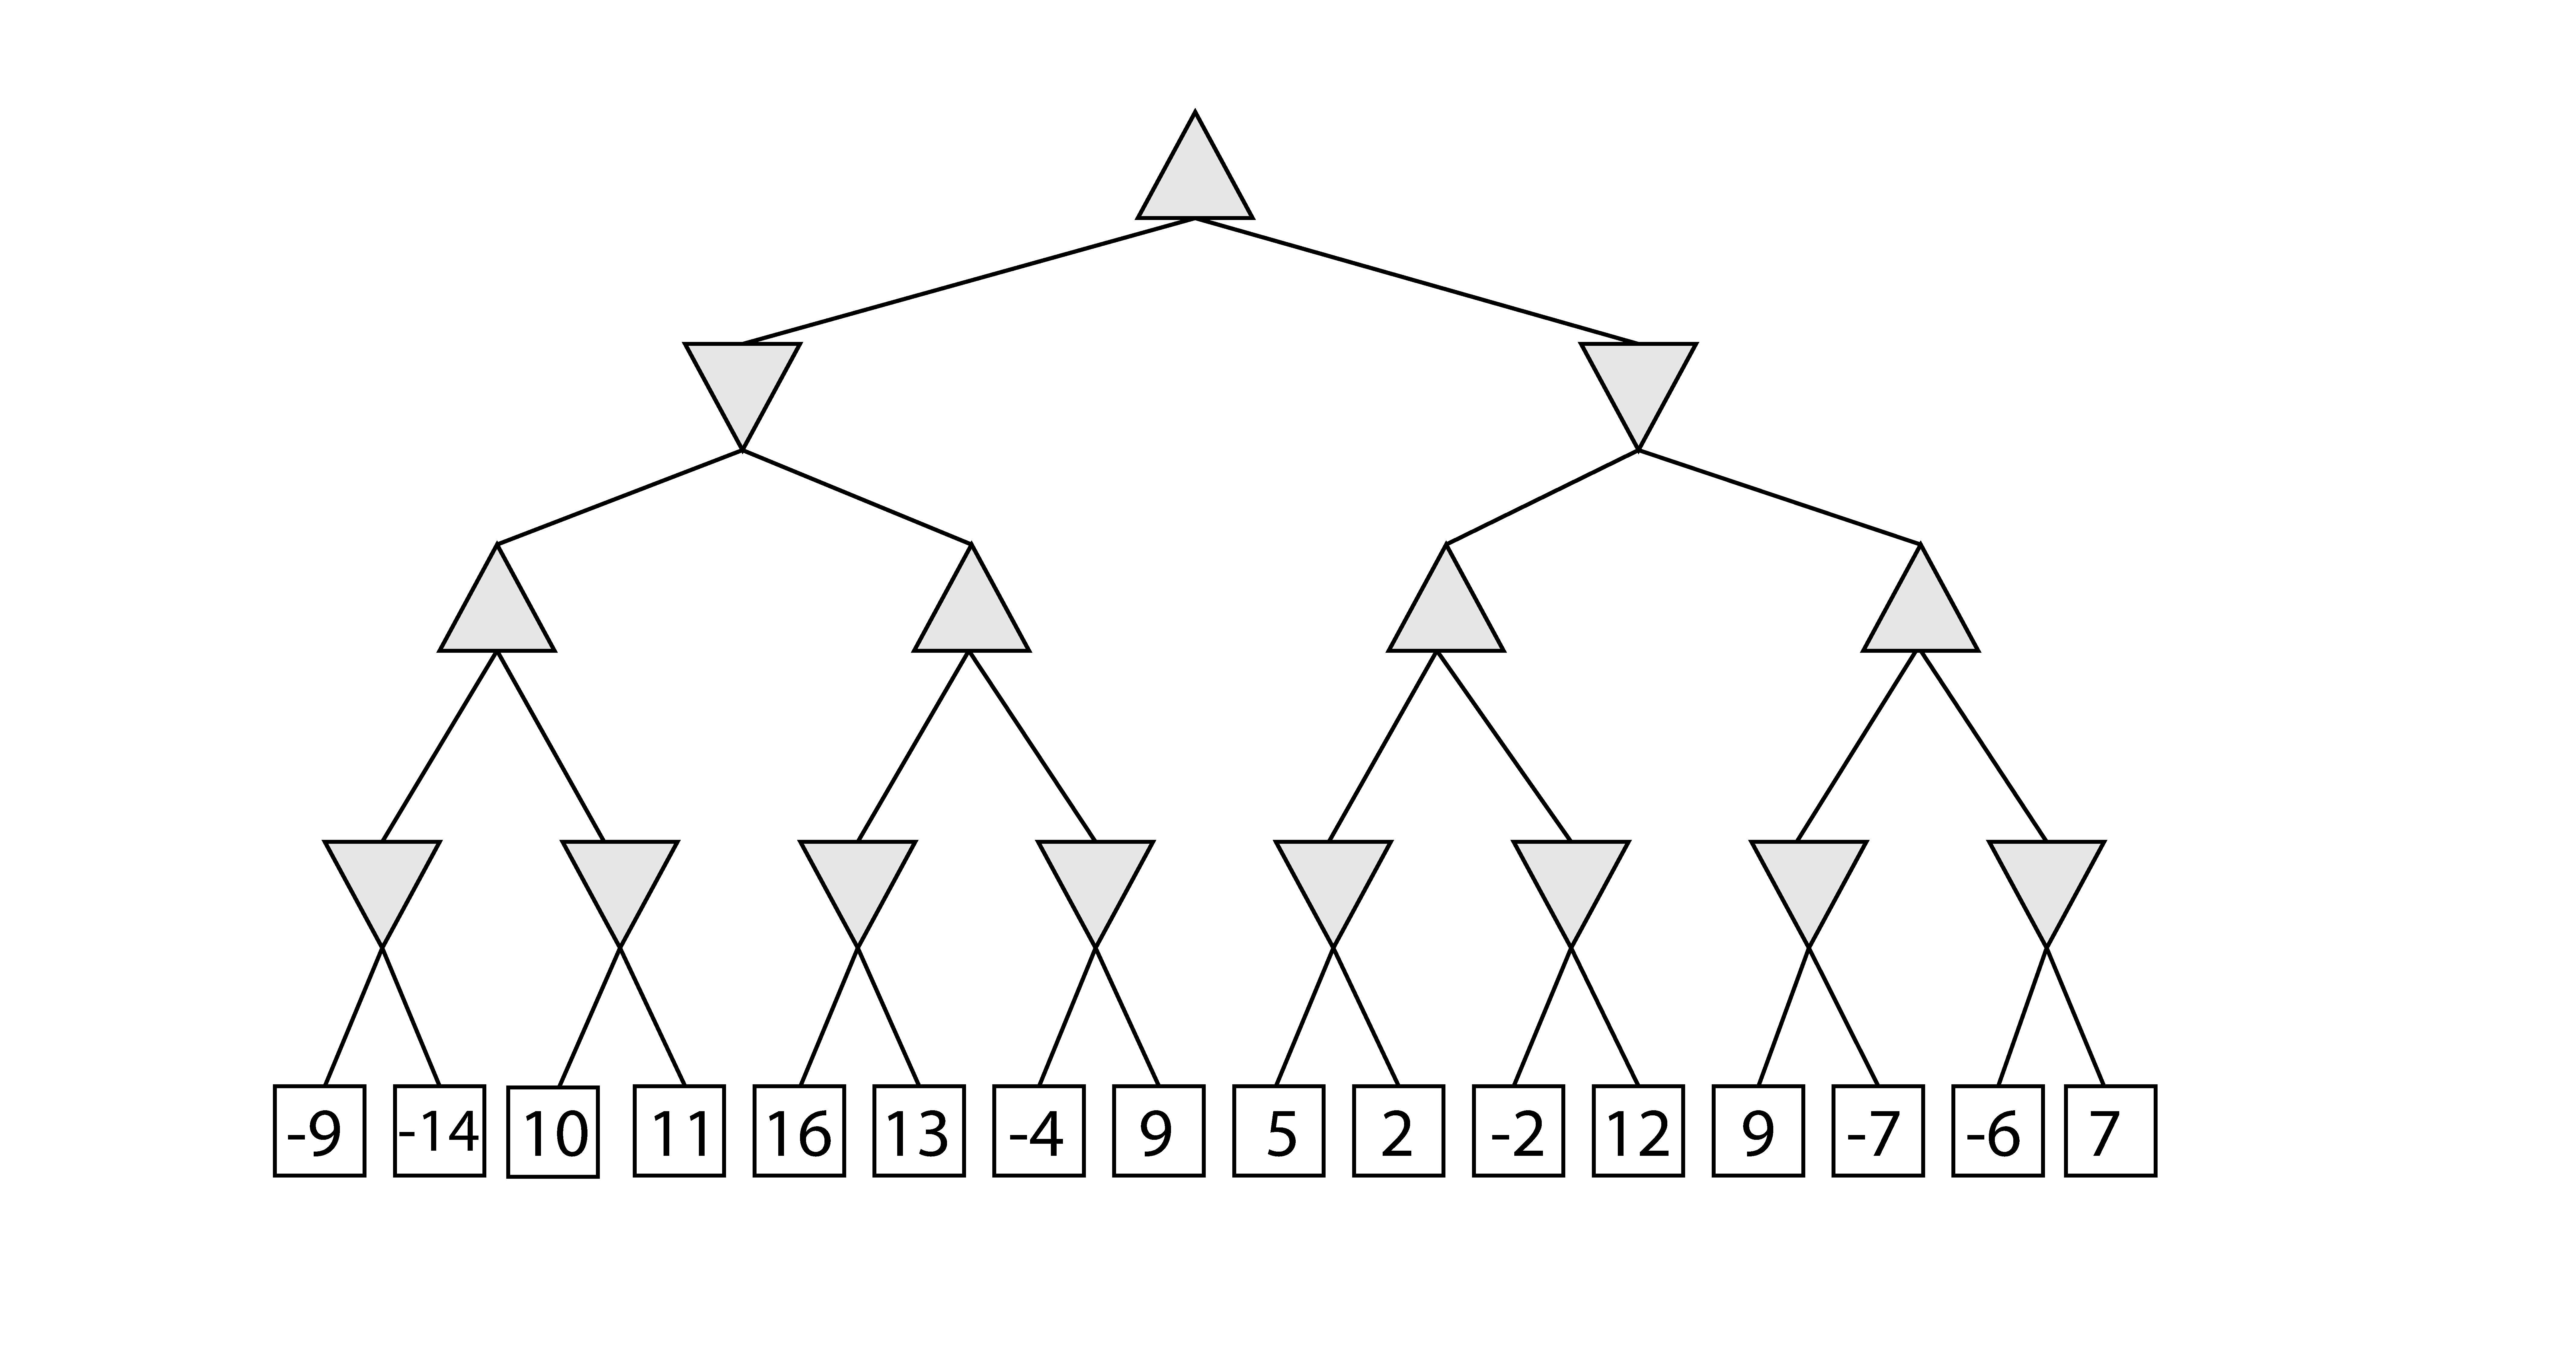
\includegraphics[width=1.25\textwidth]{figs/minmax}
\end{figure}
\end{center}

\newpage

\item After running the algorithm, you notice that the other player is not playing optimally. Instead, the player picks their action uniformly at random. Recompute the values of the nodes. What is the action at the root now? 

\begin{center}
\begin{figure}[h!]
\centering
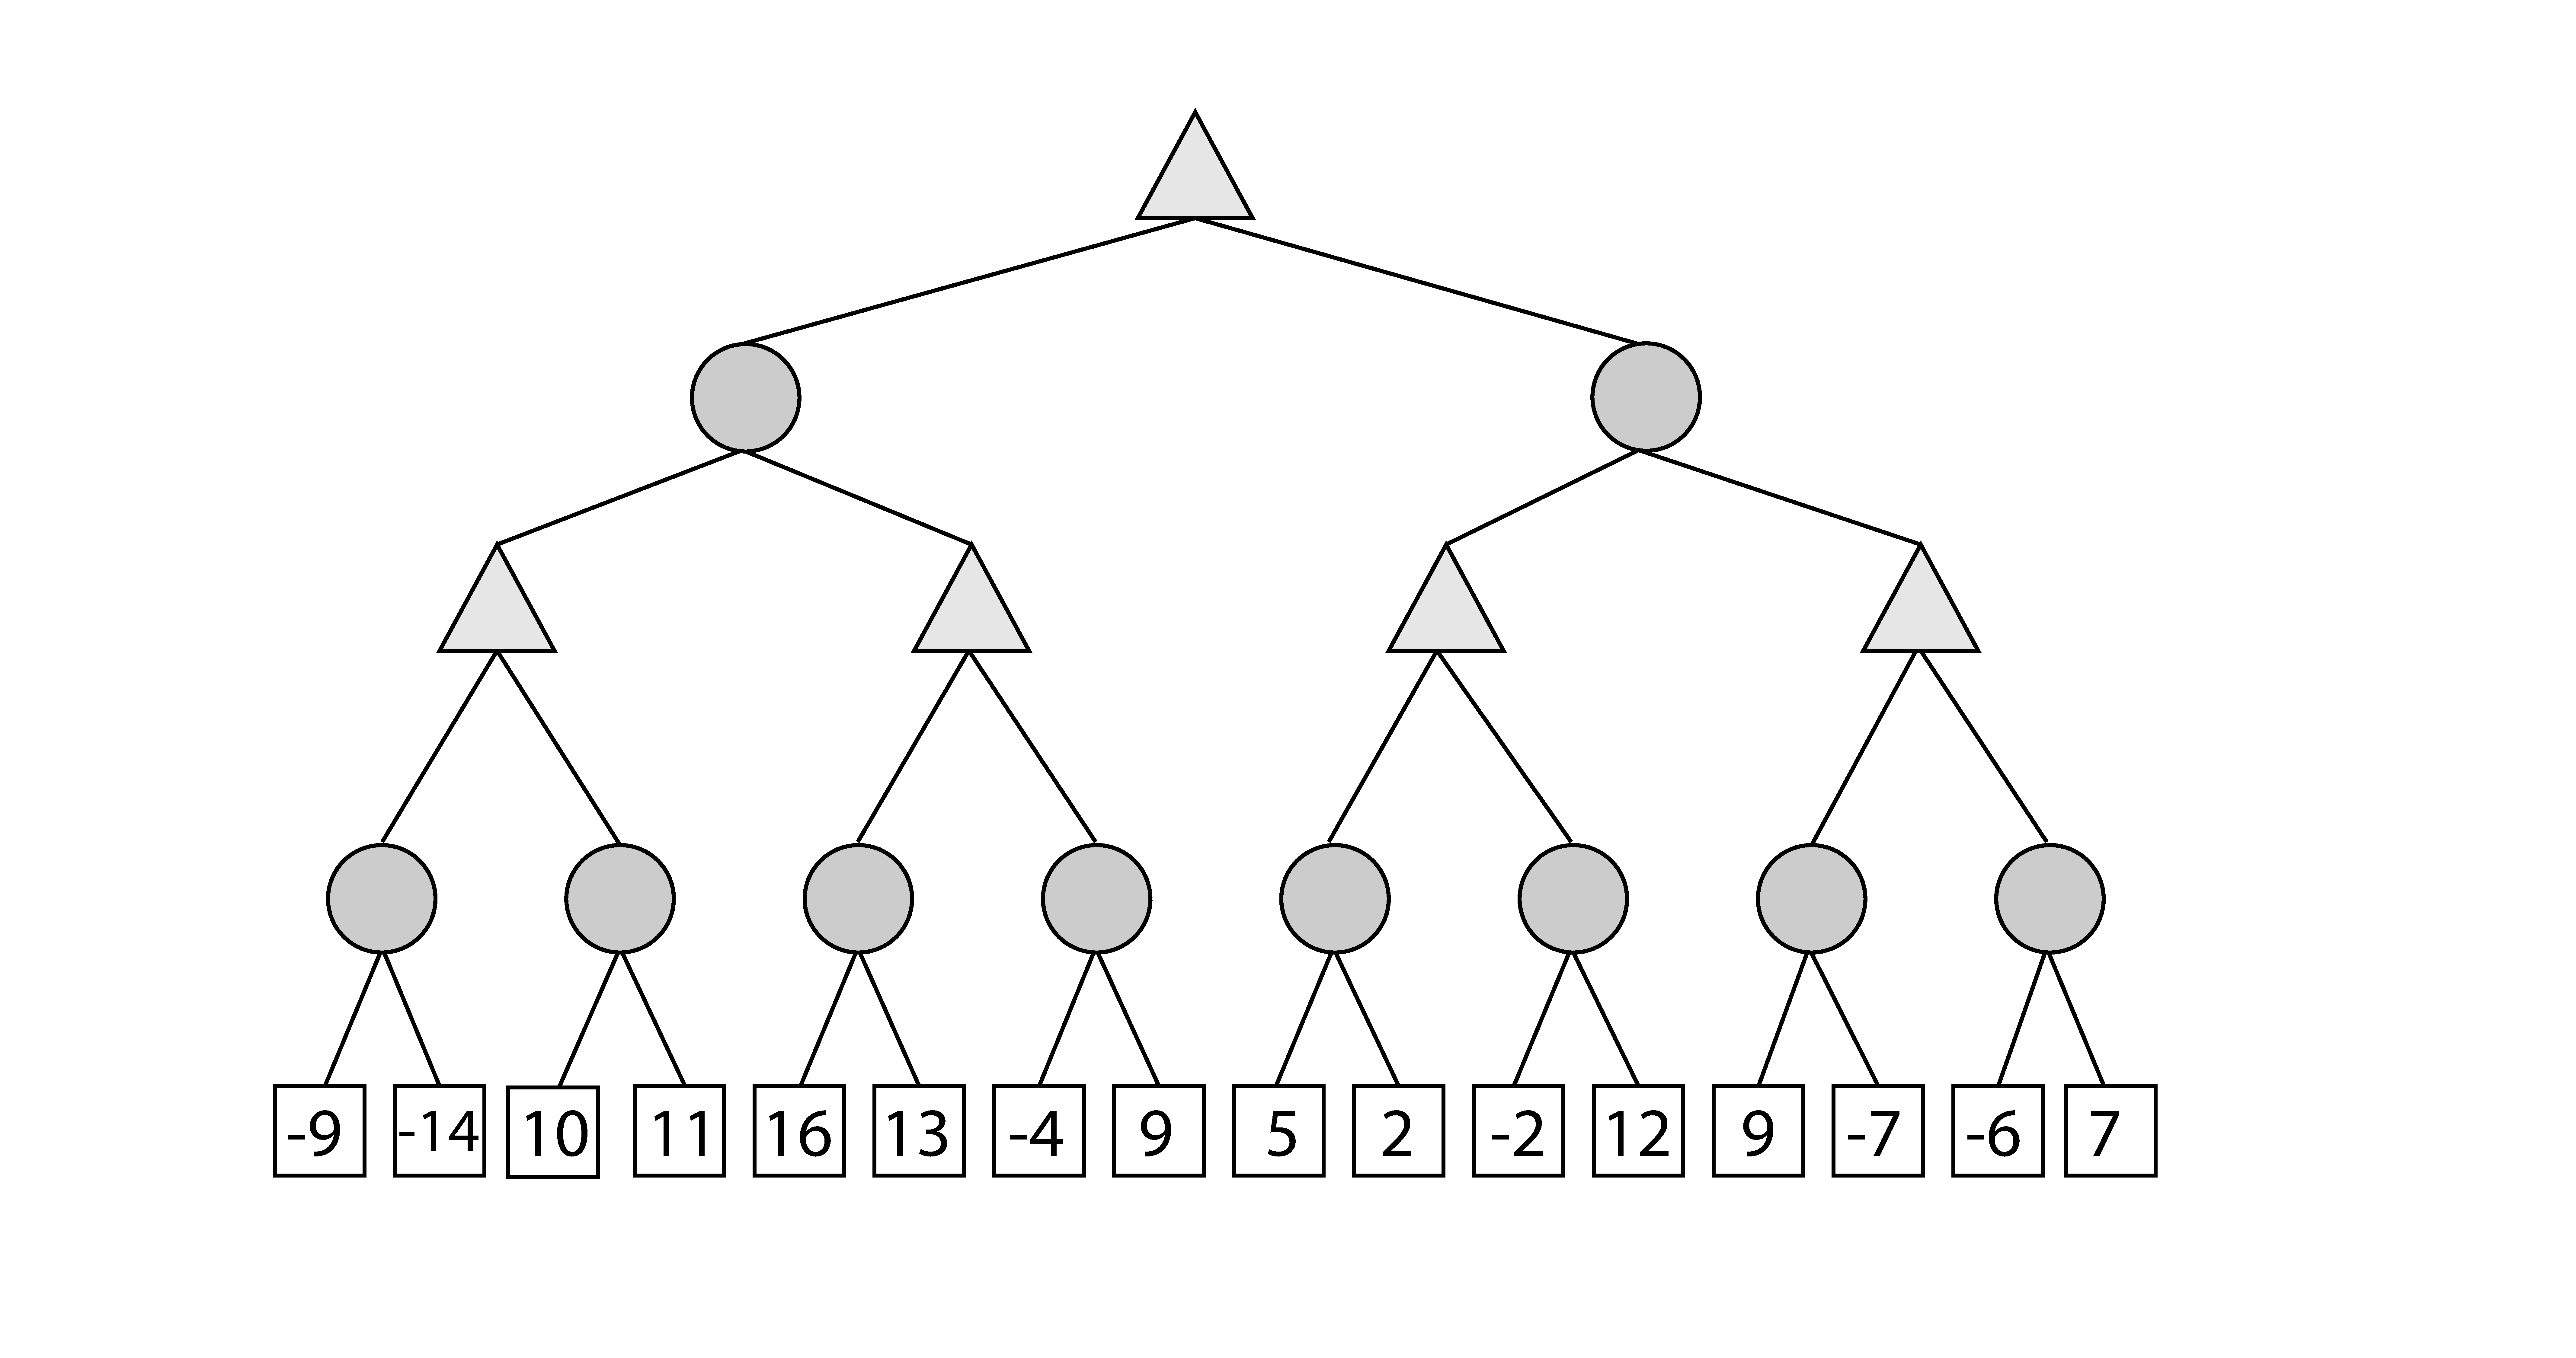
\includegraphics[width=1.25\textwidth]{figs/expectimax}
\end{figure}
\end{center}


\item Your computer can only use 1MB of memory while running the algorithm. A single node takes 10B to store. Given a branching factor of 3, Compute an upper bound on the depth of a tree that your computer can conduct AB-pruning on.

\vspace{10em}
% \textcolor{blue}{AB-pruning has at worst the same complexity as Minimax. For Minimax, time complexity is $O(b^m)$ and space complexity is $O(bm)$. To compute the space limit, we have to solve 
% \begin{align*}
% 1024^2\text{B} &=3*10\text{B}*m \\
% m &= 69905
% \end{align*}
% Therefore, the maximum depth is 69905. 
% }

\item Your computer can check 10,000 nodes per second Is it feasible to solve the problem for the maximum depth within 2 minutes? If not, what strategy do you recommend instead?

\vspace{10em}
% \textcolor{blue}{The time complexity for this tree is $3 * 10^{33398}$. Even while checking $10000$ nodes a second, it is impossible to solve. Therefore, we need to do depth-limited search. You can compute the maximum depth the algorithm can search through in 2 minutes by solving
% \begin{align*}
% 3^m &= 10000 * 120
% \end{align*}
% This gives an answer $10 < m < 11$. To fully traverse the last layer, we therefore need to choose a depth of 10 for the depth-limited search. 
% }

\newpage
\item True or false. For every game tree, the utility obtained by MAX using minimax decisions against a suboptimal MIN will be never be lower than the utility obtained playing against an optimal MIN. Justify your response. 

\vspace{15em}

% \textcolor{blue}{Consider a MIN node whose children are terminal nodes. If MIN plays suboptimally, then the value of the node is greater than or equal to the value it would have if MIN played optimally. Hence, the value of the MAX node that is the MIN node’s parent can only be increased. This argument can be extended by a simple induction all the way to the root. If the suboptimal play by MIN is predictable, then one can do better than a minimax strategy. For example, if MIN always falls for a certain kind of trap and loses, then setting the trap guarantees a win even if there is actually a devastating response for MIN. Consider the tree shown below: If we know for sure that B would pick $b_1$ or $b_2$ over $b_3$, then picking $a_1$ over $a_2$ would be the correct choice.}


Can you come up with a game tree in which MAX can do still better using a suboptimal strategy against a suboptimal MIN?

\vspace{10em}
% \begin{center}
% \begin{figure}[h!]
% \centering
% \includegraphics[width=.6\textwidth]{figs/suboptimal-min}
% \end{figure}
% \end{center}

\end{enumerate}

\section{CSP}

You are designing a menu for a special event. There are several choices, each represented as a variable:
(A)ppetizer, (B)everage, main (C)ourse, and (D)essert. The domains of the variables are as follows:
\begin{itemize}
\item A: (v)eggies, (e)scargot
\item B: (w)ater, (s)oda, (m)ilk
\item C: (f)ish, (b)eef, (p)asta
\item D: (a)pple pie, (i)ce cream, (ch)eese
\end{itemize}
Because all of your guests get the same menu, it must obey the following dietary constraints:
\begin{itemize}
\item (i) Vegetarian options: The appetizer must be veggies or the main course must be pasta or fish (or both).
\item (ii) Total budget: If you serve the escargot, you cannot afford any beverage other than water.
\item (iii) Calcium requirement: You must serve at least one of milk, ice cream, or cheese.
\end{itemize}

\begin{enumerate}[(a)]
\item Draw the constraint graph over the variables

\newpage
% \textcolor{blue}{\textbf{Solution:}}

% \begin{tikzpicture}[
%         shorten >=1pt, auto, thick,
%         node distance=3cm,
%     main node/.style={circle,draw,fill=blue!20,font=\sffamily\Large\bfseries}
%                             ]
%       \node[main node] (a) at (0,0) {A};
%       \node[main node] (b) at (2,0) {B};
%       \node[main node] (d) at (2,-2) {D};
%       \node[main node] (c) at (0,-2) {C};

%       \path[every node/.style={font=\sffamily\small}]
%         (a) edge node {} (b)
%         (a) edge node {} (c)
%         (b) edge node {} (d);
% \end{tikzpicture}


\item Imagine we assign $A=e$. Cross out the eliminated values to show the domains of the variable after forward checking
\begin{center}
\begin{tabular}{|c|c|c|c|}
\hline
A &  & e &  \\
\hline
B& w & s  & m  \\
\hline
C& f & b  & p  \\
\hline
D& a & i  & ch  \\
\hline
\end{tabular}
\end{center}

% \textcolor{blue}{The values s, m, and b should be crossed off. "s" and "m" due to constraint (ii), and "b" due to (i).}

\item Imagine again that $A=e$. Cross out the eliminated values after enforcing arc consistency.
\begin{center}
\begin{tabular}{|c|c|c|c|}
\hline
A &  & e &  \\
\hline
B& w & s  & m  \\
\hline
C& f & b  & p  \\
\hline
D& a & i  & ch  \\
\hline
\end{tabular}
\end{center}

% \textcolor{blue}{The values s, m, b, and a should be crossed out.  The first three are crossed off for the same reasons as above, and “a” is eliminated because there is no value for (B) that is compatible with “a” (based on constraint (iii)).}

\item Give a solution for this CSP or show that none exists. 

\vspace{5em}
% \textcolor{blue}{There are multiple solutions. One of them is A=e, B=w, C=f, and D=i.}

\item Define in your own words the terms constraint, backtracking search, arc consistency, backjumping, min-conflicts, and cycle cutset.

\newpage
% \textcolor{blue}{A \textbf{constraint} is a restriction on the possible values of two or more variables. For example, a constraint might say that A = a is not allowed in conjunction with B = b. \\
% \textbf{Backtracking search} is a form of depth-first search in which there is a single representation of the state that gets updated for each successor, and then must be restored when a dead end is reached. \\
% A directed arc from variable A to variable B in a CSP is \textbf{arc consistent} if, for every value in the current domain of A, there is some consistent value of B. \\
% \textbf{Backjumping} is a way of making backtracking search more efficient, by jumping back more than one level when a dead end is reached.\\
% \textbf{Min-conflicts} is a heuristic for use with local search on CSP problems. The heuristic says that, when given a variable to modify, choose the value that conflicts with the fewest number of other variables. \\
% A \textbf{cycle cutset} is a set of variables which when removed from the constraint graph make it acyclic (i.e., a tree). When the variables of a cycle cutset are instantiated the remainder of the CSP can be solved in linear time.}

% SK--this one might be more trouble than it's worth
% \item For general CSPs, will enforcing arc consistency after an assignment always prune at least as
% many domain values as forward checking? Briefly explain why or why not.

% \textcolor{blue}{Two answers are possible:\\
% Yes. The first step of arc consistency is equivalent to forward checking, so arc consistency removes all values
% that forward checking does.\\
% No. While forward checking is a subset of arc consistency, after any assignment, arc consistency may have
% already eliminated values in a previous step that are eliminated in that step by forward checking. Thus,
% enforcing arc consistency will never leave more domain values than enforcing forward checking, but on a given step the forward checking could prune more values as arc consistency.}
\end{enumerate}

\section{MDP and RL}

\begin{enumerate}[(a)]
\item Suppose that we define the utility of a state sequence to be the maximum reward obtained in any state in the sequence. Show that this utility function does not result in stationary preferences between state sequences. Is it still possible to define a utility function on states such that MEU decision making gives optimal behavior?


\vspace{25em}
% \textcolor{blue}{Stationarity requires the agent to have identical preferences between the sequence pair [$s_0, s_1, s_2, \ldots$], [$s'_0, s'_1, s'_2, \ldots$] and between the sequence pair [$s_1, s_2, \ldots$], [$s'_1, s'_2, \ldots$]. If the utility of a sequence is its maximum reward, we can easily violate stationarity. For example,
% \begin{equation*}
% [4, 3, 0, 0, 0, \ldots] \sim [4, 0, 0, 0, \ldots]
% \end{equation*}
% but 
% \begin{equation*}
% [3, 0, 0, 0, \ldots] \succ [0, 0, 0, \ldots]
% \end{equation*}
% We can still define $V^\pi(s)$ as the expected maximum reward obtained by executing $\pi$ starting in $s$. The agent’s preferences seem peculiar, nonetheless. For example, if the current state $s$ has reward $R_{\max}$, the agent will be indifferent among all actions, but once the action is executed and the agent is no longer in $s$, it will suddenly start to care about what happens
% }

\item Can all MDPs be solved using expectimax search? Justify your answer

\vspace{8em}
% \textcolor{blue}{No, MDPs with self loops lead to infinite expectimax trees. Unlike search problems, this issue cannot be addressed with a graph-search variant.}

\item Let's consider a two-player MDP that correspond to a zero-sum, turn-taking game. Let the players be $A$ and $B$, and let $R(s)$ be the reward for player $A$ in state $s$. (The reward for $B$ is always equal and opposite.). Let $V^*_A(s)$ be the utility of state $s$ when it is $A$’s turn to move in $s$, and let $V^*_B(s)$ be the utility of state $s$ when it is $B$’s turn to move in $s$. All rewards and utilities are calculated from $A$’s point of view (just as in a minimax game tree). Write down the definitions of $V^*_A(s)$ and $V^*_B(s)$ in terms of expected future utility. 

\vspace{8em}
% \textcolor{blue}{\begin{align*}
% V^*_A(s) &= \max_{a} \sum_{s'} P(s'|s,a)[R(s,a,s') + \gamma V^*_B(s')]\\
% V^*_B(s) &= \min_{a} \sum_{s'} P(s'|s,a)[R(s,a,s') + \gamma V^*_A(s')]
% \end{align*}}

\item Explain how to do two-player value iteration with these equation. Additionally, state how to check whether the algorithm has converged. 

\newpage
% \textcolor{blue}{To do value iteration, we simply keep track of twice as many values - once for $A$ and once for $B$. We can use the equations from the previous task and apply them in alternation. The process terminates when the utility vector for one player is the same as the previous utility vector for the same player (i.e., two steps earlier). (Note that the policies and utilities for the two players might not be the same.)}


\begin{center}
\begin{figure}[h!]
\centering
\includegraphics[width=.25\textwidth]{figs/small-2-player}
\caption{The starting position for a simple game. The two players take turns moving, and each player must move his token to an open adjacent space in either direction. If the opponent occupies an adjacent space, then a player may jump over the opponent to the next open space if any. (For example, if $A$ is on $3$ and $B$ is on $2$, then A may move back to 1.) The game ends when one player reaches the opposite end of the board. If player A reaches space 4 first, then the value of the game to $A$ is $+1$; if player $B$ reaches space 1 first, then the value of the game to $A$ is $−1$.}
\end{figure}
\end{center}

\item Consider the game described in the figure above. Draw the state space (rather than the game tree), showing the moves by $A$ as solid lines and moves by $B$ as dashed lines. Mark each state with $R(s)$. You will find it helpful to arrange the states $(s_A,s_B)$ on a two-dimensional grid, using $s_A$ and $s_B$ as “coordinates.”

\vspace{15em}
% \textcolor{blue}{\textbf{Solution:}}
% \begin{center}
% \begin{figure}[h!]
% \centering
% \includegraphics[width=.25\textwidth]{figs/state-space}
% \end{figure}
% \end{center}


\item Now apply two-player value iteration to solve this game, and derive the optimal policy. Use a $\gamma$ of 1 for the derivation.

\newpage
% \textcolor{blue}{\textbf{Solution:}}
% \begin{center}
% \begin{figure}[h!]
% \centering
% \includegraphics[width=.8\textwidth]{figs/value-it}
% \end{figure}
% \end{center}

\item When using features to represent the Q-function is it guaranteed that the feature-based $Q$-learning finds the same optimal $Q^∗$ as would be found when using a tabular representation for the $Q$-function?

\vspace{8em}
% \textcolor{blue}{No, if the optimal $Q$-function $Q^∗$ cannot be represented as a weighted combination of features, then the feature-based representation would not have the expressive power to find it.}

\item Why is temporal difference (TD) learning of Q-values (Q-learning) superior to TD learning of values?

\vspace{8em}
% \textcolor{blue}{Because if you use temporal difference learning on the values, it is hard to extract a policy from the learned values. Specifically, you would need to know the transition model $T$. For TD learning of Q-values, the policy can be extracted directly by taking $\pi(s) = \text{argmax}_a Q(s, a)$.}

\end{enumerate}

\end{document}